% !TEX root = ../../../../main/numb3rs_activities.tex
\newpage
\phantomsection
\addcontentsline{toc}{subsection}{110: Dirty Bomb \label{ep110}}
\ep{110: Dirty Bomb}
\setcounter{activity}{0}

In this episode there was a discussion about triangulation and there was a scene where Charlie explains the prisoner's dilemma to three prisoners in the hope that it will make one of them confess. \\


% Triang.
\ltLarge{Triangulation}


In this episode a truckload of radioactive waste has been hijacked and Charlie uses triangulation of the radiation the waste emits to find where it is. This is mathematically similar to trying to find a lightbulb in a very large field (without moving). If you are standing in a field, then you will be able to see the lightbulb but you won't be able to tell how far away it is. This means you know that it lies somewhere on a particular line that goes through you, which probably wouldn't be particularly useful, since to find the lightbulb without gathering more information you would have to walk along the entire line to get to the lightbulb.

	\begin{figure}[H]
	\centering
	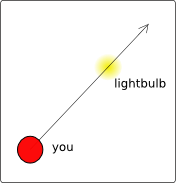
\includegraphics[width=0.30\textwidth]{../sections/seasons/season1/110/images/drawing1.png} 
	\end{figure}


However, let's say you have a friend in the field and both you and your friend have lightbulbs and radios. Then you can report to each other the angle between the friend's lightbulb and the other lightbulb. Is this enough to find the other lightbulb? Not quite, because there is no angle-angle theorem in geometry. In other words, if you adapt coordinates so that you are at the origin, then if you double the distances of the other lightbulb and your friend from the origin, both the angles that you and your friend measure will be the same. The only way to fix this is to measure the distance between you and your friend.


	\begin{figure}[H]
	\centering
	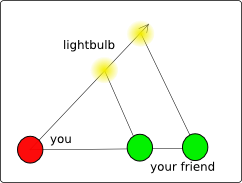
\includegraphics[width=0.4\textwidth]{../sections/seasons/season1/110/images/drawing2.png} 
	\end{figure}


Of course, if you are unlucky there will be a problem with this. There is a chance that the lightbulb will lie on the line between you and your friend. If this is the case, it would be impossible for you and your friend to tell where on the line the lightbulb is. This can be fixed, however, by adding a third friend. If the three friends make sure they aren't all standing on a single line, then they can always find the lightbulb.


	\begin{figure}[H]
	\centering
	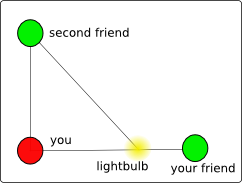
\includegraphics[width=0.4\textwidth]{../sections/seasons/season1/110/images/drawing3.png} 
	\end{figure}


\activity{Let's say you are standing on the coordinates $(0,0)$ (the origin), your first friend is standing at $(1,0)$, and your second friend is standing at $(0,1)$. Also, assume the lightbulb is in the first quadrant so that both its coordinates are positive.
	\begin{figure}[H]
	\centering
	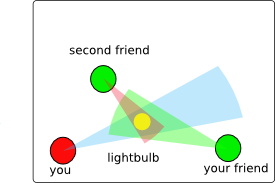
\includegraphics[width=0.5\textwidth]{../sections/seasons/season1/110/images/drawing4.png} 
	\end{figure}
\begin{enumerate}[1.]
\item If the angle you see between your first friend and the lightbulb is $45^\circ$ and the angle he sees between you and the lightbulb is $90^\circ$, where is the lightbulb?
\item If both your friends report an angle of $90^\circ$ between you and the lightbulb, where is the lightbulb?
\item What if both your friends report an angle of $0^\circ$ between you and the lightbulb?
\end{enumerate}
}


Of course, in the real world you can't measure exactly what the angle is between your friend and the lightbulb. Any measurement has errors, so all that you will actually be able to say is that the lightbulb is very likely to lie inside a cone whose point is your location. The more accurate your measurement is, the skinnier the cone will be. 


\activity{In the above picture with errors in measurements, which friend would be better to ask about his estimate of the angle between you and the lightbulb? Why? [Assume each friend has the same error in measuring angles.] }


\tangent{The GPS, or \bref{Global Positioning System}{https://en.wikipedia.org/wiki/Global_Positioning_System}, uses a similar method to determine the exact location of a small handheld unit. Instead of having friends in a field the system has satellites in the sky that have very precise clocks in them. The handheld unit receives signals from the satellites saying what time they think it is and their current location, which allows the handheld unit to calculate the distance from it to each of the satellites. Then the handheld unit is able to mathematically determine its location. Interestingly, the clocks are so accurate that they are able to detect effects from general relativity, and correcting for these effects leads to improvements in positional measurement of tens of meters.}


% Prisoner
\ltLarge{The Prisoner's Dilemma}


In this episode, Charlie refers to the Prisoner's Dilemma, which is a particular game that shows that if the players in a game are only looking out for themselves and not colluding with the other players, then the results of the game might be worse for everyone involved. Here's how it works. Suppose that there are two prisoners that were involved in the same crime, and for the police to successfully convict either one of them, they need the testimony of the other one. If neither prisoner testifies, then they will each serve 2 months on minor charges. If one testifies and the other doesn't, then the testifier will go free and the other will serve 12 years. However, if both testify, then each will get 8 years. Now it's obvious that if the prisoners can collude and trust each other, neither will testify. This result would be the best possible outcome in the sense that the total time served would be minimized. However, if each prisoner only acts in his own interest, both of them will testify. This is because if one prisoner testifies, the outcome for him is better than if he didn't testify no matter what the other person does. This situation can be conveniently described in a table where the first number listed is the incarceration time (called a payoff in game theory) of the first prisoner and the second number is the incarceration time of the second prisoner. \\

	\begin{table}[H]
	\centering
	\begin{tabular}{c|c|c}
	 & Prisoner 2 Testifies & Prisoner 2 is Silent \\ \hline
	 Prisoner 1 Testifies & 8, 8 & 0, 12 \\ \hline
	 Prisoner 1 is Silent & 12, 0 & 2 months, 2 months
	\end{tabular}
	\end{table}


\activity{
\begin{enumerate}[1.]
\item If we have the following table, what are some conditions on the numbers $a, b, c, d$ so that the argument given above still works and the equilibrium solution is the lower right hand square?
	\begin{table}[H]
	\centering
	\begin{tabular}{c|c|c}
	 & Prisoner 2 Testifies & Prisoner 2 is Silent \\ \hline
	 Prisoner 1 Testifies & $a,a$ & $b,c$ \\ \hline
	 Prisoner 1 is Silent & $c,b$ & $d,d$
	\end{tabular}
	\end{table}
\item Use reasoning similar to the argument above to figure out the equilibrium choices for the following game. (The left number is the payoff for player 1, and for this game bigger numbers are better.)
	\begin{table}[H]
	\centering
	\begin{tabular}{c|c|c|c}
	 & Player 2, Choice $A$ & Player 2, Choice $B$ & Player 2, Choice $C$ \\ \hline
	 Player 1, Choice $A$ & 4, 9 & 6, 4 & 1, 9 \\ \hline
	 Player 1, Choice $B$ & 5, 3 & 9, 5 & 5, 2 \\ \hline
	 Player 1, Choice $C$ & 1, 7 & 15, 12 & 10, 8 
	\end{tabular}
	\end{table}
\item Will similar reasoning work for the following game? Why or why not? Is there an equilibrium solution? (An equilibrium solution is a choice for player $A$ and $B$ such that given knowledge of player $B$'s choice, player $A$ wouldn't want to change his choice, and vice versa.)
	\begin{table}[H]
	\begin{tabular}{c|c|c}
	 & Prisoner 2 Testifies & Prisoner 2 is Silent \\ \hline
	 Prisoner 1 Testifies & $2,-2$ & $-2,2$ \\ \hline
	 Prisoner 1 is Silent & $-2,2$ & $2,-2$
	\end{tabular}
	\end{table}
\end{enumerate}
}